The concepts presented in this chapter aims to introduce a review of the literature with relevant works on blur segmentation and multifocus image fusion. The methods in both fields are somehow related, as the output of a blurry region segmentation is the input for image fusion. The blur segmentation is mostly related to transform domain methods, but some of them also have simpler mathematical tools. In a nutshell, all of them are related to the standard image processing stages: pre-processing, particular operations, feature vector extraction and analysis. 

The literature review of multifocus image fusion shows that the trend is to use either more sophisticated methods or classic and well-known methods with enhancements in order to achieve the lossless image. Instead of just creating a blur map, the fusion works aim for a specific task which will presume that the image is at its best quality possible. 

\section{Blur Segmentation}

The main challenge of this project is to split the image between sharp parts and the blurred parts. The purpose of image segmentation techniques, according to \citeonline{petrou2010image}, is to extract regions that divide the image into sets of pixels with a common feature or characteristic. The extracted regions may be objects of interest for future processing or analysis. In our work, the objective is to obtain regions that were affected by the degradation process of blurring.

In agreement with \citeonline{uma2016comparison}, the segmentation of the unfocused regions of an image may be necessary for performing post-processing and restoration processes without affecting the sharp regions. This would allow feature extraction on these clear regions, which leads to a broad variety of analysis techniques. One of the principal elements of images that loses identity with the blurring process is the edge. Regardless of properties such as thickness, shape or irregularity, the edges consist of transitions that exhibit discontinuities of intensity. Edge detectors are mathematical operations capable of retrieving such discontinuities, which are identified as blur points and contrast differences \cite{barat2004segmentation}.

There are many techniques to obtain a map of blurry and sharp regions and many are based on solid mathematical concepts. In the next sections, the most relevant ones will be described: Haar Wavelets \cite{liang2017automatic}, Higher Order Statistics \cite{lee2014blurred}, Discrete Cosine Transform Coefficients \cite{taiebeh2017automatic} and Singular Value Decomposition \cite{su2011blurred}.

\subsection{Wavelet-based Segmentation}

\citeonline{liang2017automatic} proposed a Haar wavelet transform-based algorithm for blur detection and segmentation. The algorithm consists of blurring the image with a known blur kernel before performing the transform decomposition. This is due to the fact that there is a significant loss of detail after segmentation, which does not occur with such intensity if the image again undergoes a blurring process. This process can be done using a simple convolution by a Gaussian filter.

Next, the difference between the initial image and the convolved one is estimated. The result of this operation is the partially blurred image, and the third-order transform is applied
in blocks of 16x16 pixels around each pixel. Each block is decomposed into three sub-blocks of
$k = \{1, 2, 3\}$ order, denoted by $\{BH_k, BV_k, BD_k \}$, which stands for horizontal, vertical and diagonals, respectively. For all orders, the $L_p$ norm of each nine components of the block, as well as the attenuation ratio $a_k$ between the components of the same block in the image test and the convolved image. The amount of blur on any pixel $(i, j)$ is given by the product of the attenuation ratios of the three orders, as presented in equations \ref{eqn:blurriness} and \ref{eqn:blurriness_norm}:

\begin{equation}
\label{eqn:blurriness}
a_k(i,j) =
    \frac
        {
            \Big\{
                ||BH_k||_p + ||BV_k||_p + ||BD_k||_p
            \Big\}
            \Big|_{T_r}
        }
        {
            \Big\{
                ||BH_k||_p + ||BV_k||_p + ||BD_k||_p
            \Big\}
            \Big|_T
        }
\end{equation}

\begin{equation}
\label{eqn:blurriness_norm}
a(i,j) = \prod_{k=1}^3a_k(i,j)
\end{equation}

The resulting $a(i, j)$ value is normalized on the $[0,1]$ interval. The closer to 1, the greater the blurriness of the block on the test image; he closer to zero, the sharper the block.

\subsection{Higher Order Statistics-based Segmentation}

The statistical approach to blur segmentation proposed by \citeonline{lee2014blurred} consists
in extracting two features from the image: the \sigla{GM}{Gradient Magnitude} and the directional coherence. Higher Order Statistics based signal analysis is a tool for handling non-gaussian signals \cite{mitra2000nonlinear}. One of these techniques consists in computing the GM \cite{lee2014blurred}, that emphasizes the most intense discontinuity edges, suppresses the less intense ones and reduces noise. The framework to compute the GM is described by the equation \ref{eqn:GM} below.

\begin{equation}
\label{eqn:GM}
GM(i) = \log 
    \Bigg[
        \frac{1}{N_{P_i}}
            \sum_{j \in P_i} 
            \Bigg\{\sqrt{ \frac{I_x(j)^2 + I_y(j)^2}{2}} \Bigg\}^k
    \Bigg]
\end{equation}

\noindent where $I_x$ and $I_y$ are values that represent the intensity gradient in vertical and horizontal directions, respectively. $P$ represents the considered region in an iteration, centered on the $i-th$ pixel, and $N$ represents the number of pixels in $P$. The $k$ value indicates the statistical order.

\sigla{DC}{Directional Coherence} is a measure of local similarities of a scene. It can be computed, according to \citeonline{lee2014blurred}, by applying the \sigla{ST}{Structural Tensor}, which divides the dominant directions and the coherence's directions in the local region, as depicted by equation \ref{eqn:ST}:

\begin{equation}
\label{eqn:ST}
ST(i) =
    \begin{bmatrix}
        \sum_{j \in P_i}I_x(j)^2  & \sum_{j \in P_i}I_x(j) + I_y(j) \\
        \sum_{j \in P_i}I_x(j) + I_y(j) & \sum_{j \in P_i}I_y(j)^2 
    \end{bmatrix}
\end{equation}

\noindent ($I_x$, $I_y$, $P$ and $N$ are the same as described in Equation \ref{eqn:GM}). The eigenvalues of the ST tensor specify the degree of the anisotropy of the gradient distribution in $i-th$ region. Finally, equation \ref{eqn:DC} defines the directional coherence.

\begin{equation}
\label{eqn:DC}
DC(i) =
    \Bigg(
        \frac{\lambda_1 - \lambda_2}{\lambda_1 + \lambda_2}
    \Bigg)^2
\end{equation}

\noindent where $\lambda_{1}$ and $\lambda_{2}$ are the eigenvalues of the $ST$ matrix. After obtaining the feature vectors, it is possible to use a classifier - a function or a set of them, which labels the elements in distinct classes - and define whether each pixel is blurry or not. If prior information is provided to the classifier, it will characterize an example of supervised learning; otherwise, it will need to be able to
infer similarities within the sample from the feature vectors, consisting in an unsupervised learning procedure. The \sigla{SVM}{Support Vector Machine} classifier can be trained and applied to determine the blurry and sharp sets of pixels.

\subsection{Discrete Cosine Transform Coefficients Based Segmentation}

The procedure which \citeonline{taiebeh2017automatic} proposed also takes into account the fact that blurred regions, before and after a second similar degradation process, have small differences when compared; besides, the differences between the sharp regions on the same metric are relevant. This peculiarity can also be verified in the \sigla{DCT}{Discrete Cosine Transform} domain: most of the high frequency coefficients are lost and the difference quoted above may be used to estimate the amount of blur in the image. 

The DCT is an important mathematical operation, commonly used in data compression and signal processing, which takes sets of values and outputs transform coefficients; its two-dimensional version is executed in blocks (small sets of pixels) and is shown by equation \ref{eqn:dct} \cite{salomon2007data}:

\begin{equation}
    \label{eqn:dct}
    G_{ij} = \sqrt{\frac{2}{m}}
             \sqrt{\frac{2}{n}}
             C_{i} C_{j}
             \sum_{x=0}^{n-1}
             \sum_{y=0}^{m-1}
             p_{xy}
             \cos 
                \Bigg[
                \frac
                {(2y + 1)j\pi}
                {2m}
                \Bigg]
            \cos 
                \Bigg[
                \frac
                {(2x + 1)i\pi}
                {2n}
                \Bigg]
\end{equation}

\begin{align*}
C_{i} =
\begin{cases} 
    \frac{1}{\sqrt{2}} & \text{$i = 0$,} \\
    1 & \text{$i > 0$},
\end{cases}
&&
i\in \mathbb{N} \mid 0\leq i < n
&&
C_{j} =
\begin{cases} 
    \frac{1}{\sqrt{2}} & \text{$j = 0$,} \\
    1 & \text{$j > 0$},
\end{cases}
&&
j\in \mathbb{N} \mid 0\leq j < m
\end{align*}

\noindent where $p_{xy}$ is the matrix which represents the image, $m$ and $n$ are the image dimensions. As described in the equation \ref{eqn:lp_norm_ratio}, the blur metric $\beta$ consists of the quotient between the $L_p$ norm of the original blurred image coefficients and the ones from the reblurred image.

\begin{equation}
\label{eqn:dct_image}
	\mathbf{D} = DCT(\mathbf{I})
\end{equation}

\begin{equation}
\label{eqn:dct_reblurred_image}
	\mathbf{D}_b = DCT(\mathbf{I}_b)
\end{equation}

\begin{equation}
\label{eqn:lp_norm_ratio}
	\beta(\mathbf{I}) = \frac{||\mathbf{D}_b||_p}{||\mathbf{D}||_p}
\end{equation}

\noindent where $\mathbf{I} \in \mathbb{R}^{2}$ is the original image and $\mathbf{I}_b \in \mathbb{R}^{2}$ is the re-blurred image with a low-pass filter (mean filter), $\mathbf{D} \in \mathbb{R}^{2}$ and $\mathbf{D}_b \in \mathbb{R}^{2}$ are the discrete cosine transforms of $\mathbf{I}$ and $\mathbf{I}_b$, respectively. The $L_p$ norm is defined by the equation \ref{eqn:lp_norm}:

\begin{equation}
\label{eqn:lp_norm}
	||\mathbf{D}_b||_p = \sum_{u,v}{(|\mathbf{D}_b(u,v)|)^p}
\end{equation}

\noindent The $\beta$ value is normalized on the $[0,1]$ interval; the closer to 1, the greater the amount of blur. This measurement is applied pixel by pixel in blocks of experimentally determined sizes such as 45x45, 19x19 and 9x9. The final blur measure for each pixel is an average of the measurements of the three blocks, and provide a substantially accurate blur map.

The acquired blur map is smoothed between regions and allows to infer significant differences between the sharp and blurred ones. The segmentation process is based on the map, and uses the concept of \emph{pixon} (set of related pixels with similar properties as colour, intensity, texture, among others): the problem is based on classifying such sets of pixels. In order to create the pixel set, a blur map scan is performed in the neighbourhood of each pixel; the neighbours are joined to the pixons that have the average value closest to a certain threshold; otherwise a new pixon is created.

The pixon set extraction divides the blur map in a set of sub-regions which will be classified as blurred or sharp. The \sigla{FCM}{Fuzzy C-Means Algorithm} was used by \citeonline{taiebeh2017automatic} and consists of the following steps:

Let $M$ be the set of pixels with their respective intensities, $C$ be the number of classes (two, in this case) and $w\in \mathbb{R} \mid 1 < w < \infty$ be the fuzzy exponent.

\begin{enumerate}[label=\Roman*.]

    \item The fuzzy association functions $u_ {c, m}^{(0)}$ must be initialized with $c = {1,..., C}$ and $m = {1, ..., M}$, which are entries for an $\mathbf{U}^{(0)}$ array of $C$x$M$ dimensions;
    
    \item For each iteration $l = {1,2,3,...,L}$, the centroids ${v_ {c}}^{l}$ of each cluster are computed by means of the equation \ref{eqn:fuzzy_cluster_center}:
    
    \begin{equation}
    \label{eqn:fuzzy_cluster_center}
    	v_{c}^{l} = \frac{\sum_{m=1}^{M}(u_{c,m})^{w}x_m}{\sum_{m=1}^{M}(u_{c,m})^{w}}
    \end{equation}

    \item Update the $\mathbf{U}^{(l)}$ array through the equation \ref{eqn:update_matrix}:
    
    \begin{equation}
    \label{eqn:update_matrix}
    	u_{c,m} = \frac{1}{\sum_{i=1}^{C}\Big(\frac{d_{c,m}}{d_{i,m}}\Big)^{\frac{2}{w-1}}}
    \end{equation}
    
    \noindent where $d_{i,m}^2 = ||x_m - v_i||^2$ and $||.||$ stand for the Euclidean Norm.
    
    \item Compare $\mathbf{U}^{(l)}$ and $\mathbf{U}^{(l+1)}$. If $||\mathbf{U}^{(l)} - \mathbf{U}^{(l+1)}|| \leq \varepsilon$, the classification procedure halts; otherwise, it goes back to step II.

\end{enumerate}

\noindent The $w$ value determines the clustering imprecision; it has been empirically determined by the authors that $w = 2$ and $\varepsilon = 0.00005$ are appropriate choices.

\subsection{Singular Value Decomposition-based Segmentation}

\citeonline{su2011blurred} proposed a 
\sigla{SVD}{Singular Value Decomposition}-based blur segmentation approach. It is a Linear Algebra derived technique of great utility, in which an array can be represented by multiple matrices of rank 1 (in this case, they can be denominated \emph{eigenimages}). The matrix equation \ref{eqn:basic_svd}
illustrates the SVD procedure on an image.

\begin{equation}
\label{eqn:basic_svd}
	I = U{\wedge}V^{T}
\end{equation}

\noindent where $I$ is a matrix that represents the image, $U$ and $V$ are orthogonal arrays and $\wedge$ is a diagonal matrix, composed of multiple singular values sorted in descending order. The decomposition of the image can be represented more specifically by the equation \ref{eqn:svd}:

\begin{equation}
\label{eqn:svd}
	I = \sum_{i=1}^{n}\lambda_{i}{\mathbf{u}_i}{\mathbf{v}_i}^{T}
\end{equation}

\noindent where $\mathbf{u}_i$, $\mathbf{v}_i$ are column vectors of $U$ and $V$, and $\lambda_{i}$ are the diagonal terms of $\wedge$. This process decomposes the image into a weighted sum with a certain amount of eigenimages, where the weights are singular values. Image details are captured as if it was a compression procedure, in which only $k$ singular values are considered.

Eigenimages act as multiscale analysis tools: the first most significant eigenimages involve larger scales, which provide the coarser formats; similarly, the remaining products of the decomposition provide details. Considering the convolution of a PSF $H$ with the image $I$, the high frequencies that represent the details are lost, i.e. the small singular values will correspond to larger values after the process. A blurred image has the first most significant eigen with larger singular values. The authors in \citeonline{su2011blurred} proposed a metric quantify the degree of blurriness of the image is proposed by the equation \ref{eqn:svd_blur_metric}:

\begin{equation}
\label{eqn:svd_blur_metric}
	\beta_{1} = \frac{\sum_{i=1}^{k}\lambda_{i}}{\sum_{i=1}^{n}\lambda_{i}}
\end{equation}

\noindent where $\lambda_{i}$ is the computed singular value for the neighbourhood of a given pixel. The metric is capable of classifying all pixels of the image in blurry or sharp with a threshold-based comparison; the result of the process is also a blur map.


\section{Multifocus Image Fusion}
\label{sec:multifocus_image_fusion}

Either in microscopic or macroscopic scales, imaging devices have a finite depth of field. All the slices of the image which are blurry came from the fact that a subset of pixels might be acquired outside the boundaries of depth of field \cite{huang2007evaluation}. Therefore, it is nearly impossible to obtain a globally sharp image in microscopic scales, since the differences of heights within the surface of the sample will also be magnified and the depth of field of microscopes is usually small in those cases. Image fusion is what may provide a fully sharp image, if a stack of images is acquired with a variety of focus adjustments.

The most trivial pixel-level fusion techniques are simple mathematical operations such as the average or a weighted average of gray levels; those are capable of performing the task, but also deliver some losses in basic image features, e.g. contrast and saturation \cite{zhang2009multifocus}. Thus, there is a demand for techniques that rely on more sophisticated tools, capable of covering multiple situations: images taken in different resolutions, light conditions and exposure times, for instance. Multiscale transform approaches, e.g. wavelet domain transforms, are a good choice for the problem and provide a very flexible framework, since it depends on the chosen wavelet function \cite{pajares2004wavelet}.

Most of the methods work upon the transform domain space, but there are also some noteworthy ones which are based on different basis. The following sections will elucidate multifocus image fusion techniques such as Graph and Spatial Frequency \cite{li2008multifocus} and Wavelet Transform \cite{pajares2004wavelet}.
% and Principal Component Analysis \cite{naidu2008pixel}.

% Nonsubsampled Contourlet Transform \cite{zhang2009multifocus}

\subsection{Graph and Spatial Frequency-based Fusion}

\citeonline{li2008multifocus} proposed an approach for the multifocus image fusion task that works on the spatial domain and has two fusion stages: the image is fused with the simple average method, then a segmentation procedure is performed by means of graph algorithms; the result is a region split of the initial images, which will be fused again with a spatial frequency technique.

Let $\mathbb{G} = (\mathbb{V},\mathbb{E})$ be the representation of a undirected weighted graph, where $\mathbb{V} = \{v_{1},v_{2},...,v_{n}\}$ is the set of vertices that stands for the pixels of the image and $\mathbb{E} = \{e_{1},e_{2},...,e_{m}\}$ is the set of edges that connect each pair of nodes based on the similarity degree shown by $\mathbf{W}(i,j)$, the weight function. The Normalized Cut algorithm is responsible for dismembering the graph into two complementary sets $A$ and $B$, and its threshold value for cutting edges is defined by equation \ref{eqn:ncut_base}

\begin{equation}
\label{eqn:ncut_base}
    Ncut = 
    \frac{cut(A,B)}{assoc(A,\mathbb{V})} +
    \frac{cut(A,B)}{assoc(B,\mathbb{V})}
\end{equation}

\noindent where $cut(A,B)$ is the sum of 
weights from $A$ to $B$, $assoc(A,\mathbb{V})$ and $assoc(B,\mathbb{V})$ are the sums of weights from $A$ an $B$ to the whole graph, respectively.

Considering $T$ as a input image, $(i,j)$ as indices for nodes, $\mathbf{F}(i)$ as intensity value for node $i$, $\mathbf{X}(i)$ as the coordinates of node $i$ and $\sigma$ as a coefficient set within 10\% and 20\% of the distance range, the proposed segmentation algorithm is organized in the following steps, as shown by \cite{li2008multifocus}:
    
\begin{enumerate}[label=\Roman*.]
    \item Build the graph with the chosen distance or similarity function and build two matrices $\mathbf{W}$ and $\mathbf{D}$, where
    
    \begin{align*}
        \mathbf{W}(i,j) = 
        \exp{\frac{-||\mathbf{F}(i)-\mathbf{F}(j)||_{2}^{2}}{\sigma_{I}^{2}}} t,
        &&
        t = 
        \begin{cases}
            \exp{\frac{-||\mathbf{X}(i)-\mathbf{X}(j)||_{2}^{2}}{\sigma_{X}^{2}}} & \text{if}
            ||X(i)-X(j)||_{2} < r
            \\0 & \text{otherwise}
        \end{cases}
    \end{align*}
    
    where $r$ is a threshold to create zeroes in $\mathbf{W}$ if the nodes have a greater distance in comparison to it and $\mathbf{D}$ is the diagonal matrix of cumulative sums for each node;
    
    \item The next step consists in computing the eigenvectors of $(\mathbf{D} - \mathbf{W})\mathbf{x} = \lambda\mathbf{D}\mathbf{x}$ with the smallest eigenvalues and minimizing the $Ncut$ function in order to perform a partition on the graph;
    
    \item Finally, check the stability of the partition by comparing the ratio between minimum and maximum of the histogram of eigenvectors values to an empirically determined threshold, $0.06$.
\end{enumerate}

With the two graph representations of image regions in hands, it is now possible to apply the spatial frequency procedure to recast the image. The metric relies on two values $RF$ and $CF$ (row frequency and column frequency), computed by equations \ref{eqn:rf} and \ref{eqn:cf}:

\begin{equation}
\label{eqn:rf}
    RF = \sqrt{\frac{1}{MN}
    \sum_{M-1}^{m=0}
    \sum_{N-1}^{n=1}
    [\mathbf{F}(m,n) - \mathbf{F}(m,n-1)]^{2}}
\end{equation}

\begin{equation}
\label{eqn:cf}
    CF = \sqrt{\frac{1}{MN}
    \sum_{N-1}^{n=0}
    \sum_{M-1}^{m=1}
    [\mathbf{F}(m,n) - \mathbf{F}(m-1,n)]^{2}}
\end{equation}

\noindent where $M$ and $N$ are the dimensions of the image and $\mathbf{F}(m,n)$ is intensity value of pixel at the position $(m,n)$. The spatial frequency is obtained by equation \ref{eqn:cf}:

\begin{equation}
\label{eqn:sf}
    SF = \sqrt{(RF)^{2} + (CF)^{2}}
\end{equation}

The spatial frequency index is then computed for every region of $A$ and $B$ subgraphs, and a decision task occurs as mathematically described in equation \ref{eqn:rof}:

\begin{equation}
\label{eqn:rof}
    RoF_{i} = 
    \begin{cases}
        RoA_{i}, & SF_{i}^{A} \geq SF_{i}^{B}\\
        RoB_{i}, & SF_{i}^{A} < SF_{i}^{B}
    \end{cases}
\end{equation}

\noindent where $i$ denotes the $i$-th region that is being calculated and the SF indices stand for correspondent regions in $A$ and $B$. If there are other images on the initial set, the process occurs in iteration for each of them.

\subsection{Wavelet Transform-based Fusion}

The modus operandi proposed by \citeonline{pajares2004wavelet} with the employment of the wavelet transform is relatively simple. It consists of applying the two-dimensional DWT in order to decompose the image in four common frequency bands for wavelet transforms as show in Figure \ref{fig:filter_banks}, where $h_{0}$ is the high band, $h_{1}$ is the low band, $f(m,n)$ is the input image and $2\downarrow$ stands for the downsampling operator that reduces the input size by half. Subsequently, there are some heuristics to merge the DWT coefficients and consequently the images.

\begin{figure}[htb]
	\centering
	\caption{\label{fig:filter_banks}Two-dimensional filter bank with four frequency bands.}
	\begin{center}
	    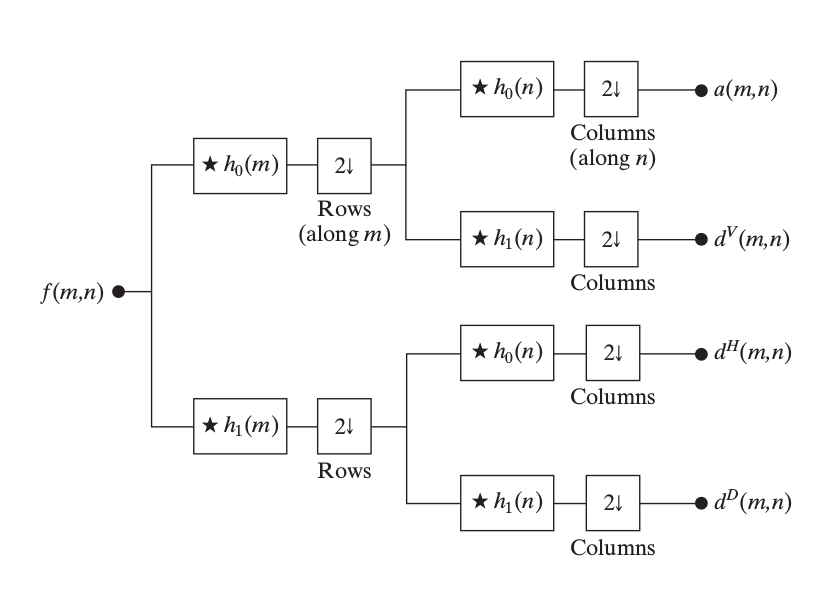
\includegraphics[scale=0.4]{images/fig11.png}
	\end{center}
	\centering
    \fdireta{gonzalez2008digital}
\end{figure}

Then, the coefficients will go through a thresholding procedure: the minimum value for taking a coefficient as significant may be obtained by the relationship of the standard deviation $\sigma$ of them all and the total size $n$ of the input: $T = \sigma\sqrt{2logn}/\sqrt{n}$. With the values from the last processing stage in hands, the fusion procedure happens with a \emph{fusion rule}, i.e. the heuristic to pick the right pixel value on each matrix in order to obtain the best fused image possible. All the values to be merged must represent the same resolution level, despite the decomposition level and the frequency band. For the multifocus image fusion, \citeonline{pajares2004wavelet} suggest the use of \sigla{CM}{Choose-Max} and \sigla{AWA}{Adaptive Weighted Average} heuristics. The CM depends on a property named activity level of the regions, represented by equation \ref{eqn:activity_level}

\begin{equation}
    \label{eqn:activity_level}
    A_{I}(p) = |D_{I}(p)|
\end{equation}

\noindent where $p = (m,n,k,l)$ is a tuple that represent a pixel in one of the decomposition levels: $m$ and $n$ indicate the spatial position in a given
frequency band, $k$ the decomposition level, and $l$ the frequency band. $D$ is a matrix with the coefficients from the decomposed image. To compute the elements that will compose the fused image, the CM procedure uses the maximum value of the same position in the two or more images, as shown by equation \ref{eqn:cm}

\begin{equation}
    \label{eqn:cm}
   CM = \max(A_{X}(p),A_{Y}(p))
\end{equation}

\noindent The AWA heuristic computes weights for each pixel with the expression in equation \ref{eqn:awa}:

\begin{equation}
    \label{eqn:awa}
   AWA = |D_{X}(p) - \Bar{D}_{X}(p)|^{a}
\end{equation}

\noindent with $\Bar{D}_{X}(p)$ representing the complementary set of positions to $D_{X}(p)$ and $a$ consisting of an exponent to modify the weight distribution. In order to finish the stack of operations and obtain the final fused image, it is only necessary to apply the \sigla{IDWT}{Inverse Discrete Wavelet Transform}.
